\documentclass{standalone}
\usepackage{tikz}
\begin{document}
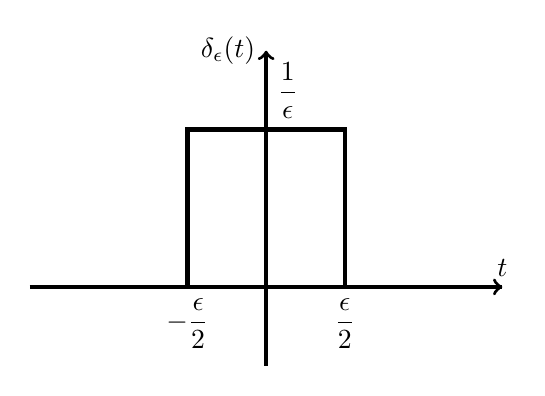
\begin{tikzpicture}[scale=2]
    \draw[->,very thick](-1.5,0)--(1.5,0)node[above]{$t$};
    \draw[->,very thick](0,-0.5)--(0,1.5)node[left]{$\delta_\epsilon(t)$};

    \draw[-, ultra thick](-1.5,0)--(-0.5,0)node[below]{$-\displaystyle\frac{\epsilon}{2}$}--(-0.5,1)--(0,1)node[above right]{$\displaystyle\frac{1}{\epsilon}$}--(0.5,1)--(0.5,0)node[below]{$\displaystyle\frac{\epsilon}{2}$}--(1.5,0);
\end{tikzpicture}
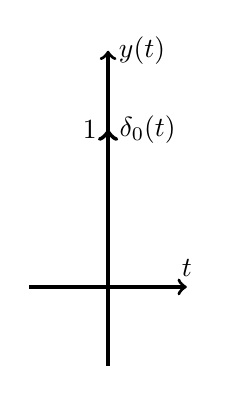
\begin{tikzpicture}[scale=2]
    \draw[->,very thick](-0.5,0)--(0.5,0)node[above]{$t$};
    \draw[->,very thick](0,-0.5)--(0,1.5)node[right]{$y(t)$};

    \draw[->,ultra thick](0,0)--(0,1)node[left]{$1$}node[right]{$\delta_0(t)$};
\end{tikzpicture}
\end{document}